\documentclass[a4paper]{article}
\date{\today}

%%%%%%%%%%%%%%%%%%%%%%%%%%%%%%%%%%%%%%%%
%%%%%%%%%%%%%%%%%%%%%%%%%%%%%%%%%%%%%%%%
%
% ENCODAGES, LANGUES, AMS ET AUTRES
%
%%%%%%%%%%%%%%%%%%%%%%%%%%%%%%%%%%%%%%%%
%%%%%%%%%%%%%%%%%%%%%%%%%%%%%%%%%%%%%%%%
%
\usepackage[T1]{fontenc}
\usepackage[utf8]{inputenc}
\usepackage{lmodern}
\usepackage[english,frenchb]{babel}
%
\frenchbsetup{StandardLists=true}
\usepackage{enumitem}
\usepackage{xspace}
\usepackage{amssymb,mathtools,pifont}
\usepackage{xcolor}
\usepackage{graphicx}
\usepackage{pdfpages}
\usepackage{float}
\usepackage{tikz}
\usetikzlibrary{trees}

%%%%%%%%%%%%%%%%%%%%%%%%%%%%%%%%%%%%%%%%
%%%%%%%%%%%%%%%%%%%%%%%%%%%%%%%%%%%%%%%%
%
% CODE HIGHLIGHTING
%
%%%%%%%%%%%%%%%%%%%%%%%%%%%%%%%%%%%%%%%%
%%%%%%%%%%%%%%%%%%%%%%%%%%%%%%%%%%%%%%%%
%
\usepackage{listings}
\definecolor{mymagenta}{rgb}{0.86,0.08,0.24}
\definecolor{mygreen}{rgb}{0,0.6,0}
\definecolor{mygray}{rgb}{0.5,0.5,0.5}
\definecolor{mymauve}{rgb}{0.58,0,0.82}
\lstset{
    language=java,
    aboveskip=3mm,
    belowskip=3mm,
    showstringspaces=false,
    columns=flexible,
    basicstyle={\small\ttfamily},
    numbers=left,
    numberstyle=\tiny\color{mygray},
    keywordstyle=\color{blue}\bfseries,
    commentstyle=\color{mygray},
    stringstyle=\color{mygreen},
    breaklines=true,
    breakatwhitespace=false,
    tabsize=3,
    captionpos=b,
    frame=trBL,
    rulecolor=\color{gray},
    literate=%Because listing does not support ut8..
    {á}{{\'a}}1 {é}{{\'e}}1 {í}{{\'i}}1 {ó}{{\'o}}1 {ú}{{\'u}}1
    {Á}{{\'A}}1 {É}{{\'E}}1 {Í}{{\'I}}1 {Ó}{{\'O}}1 {Ú}{{\'U}}1
    {à}{{\`a}}1 {è}{{\`e}}1 {ì}{{\`i}}1 {ò}{{\`o}}1 {ù}{{\`u}}1
    {À}{{\`A}}1 {È}{{\'E}}1 {Ì}{{\`I}}1 {Ò}{{\`O}}1 {Ù}{{\`U}}1
    {ä}{{\"a}}1 {ë}{{\"e}}1 {ï}{{\"i}}1 {ö}{{\"o}}1 {ü}{{\"u}}1
    {Ä}{{\"A}}1 {Ë}{{\"E}}1 {Ï}{{\"I}}1 {Ö}{{\"O}}1 {Ü}{{\"U}}1
    {â}{{\^a}}1 {ê}{{\^e}}1 {î}{{\^i}}1 {ô}{{\^o}}1 {û}{{\^u}}1
    {Â}{{\^A}}1 {Ê}{{\^E}}1 {Î}{{\^I}}1 {Ô}{{\^O}}1 {Û}{{\^U}}1
    {œ}{{\oe}}1 {Œ}{{\OE}}1 {æ}{{\ae}}1 {Æ}{{\AE}}1 {ß}{{\ss}}1
    {ű}{{\H{u}}}1 {Ű}{{\H{U}}}1 {ő}{{\H{o}}}1 {Ő}{{\H{O}}}1
    {ç}{{\c c}}1 {Ç}{{\c C}}1 {ø}{{\o}}1 {å}{{\r a}}1 {Å}{{\r A}}1
    {€}{{\euro}}1 {£}{{\pounds}}1 {«}{{\guillemotleft}}1
    {»}{{\guillemotright}}1 {ñ}{{\~n}}1 {Ñ}{{\~N}}1 {¿}{{?`}}1
}


\renewcommand{\lstlistingname}{Code}
\renewcommand{\lstlistlistingname}{Table des codes}

%%%%%%%%%%%%%%%%%%%%%%%%%%%%%%%%%%%%%%%%
%%%%%%%%%%%%%%%%%%%%%%%%%%%%%%%%%%%%%%%%
%
% MARGES, ENTÊTES ET PIEDS DE PAGE, TITRE
%
%%%%%%%%%%%%%%%%%%%%%%%%%%%%%%%%%%%%%%%%
%%%%%%%%%%%%%%%%%%%%%%%%%%%%%%%%%%%%%%%%
%
\usepackage[hcentering=true,nomarginpar,textwidth=426.8pt,textheight=650.2pt,headheight=24pt]{geometry}

\usepackage{fancyhdr}
\fancypagestyle{plain}{
\fancyhf{}
\renewcommand{\headrulewidth}{0pt}
\renewcommand{\footrulewidth}{0pt}}

\pagestyle{fancy}
\fancyhf{}
\fancyhead[L]{\rightmark}
\fancyhead[R]{ \raisebox{0.4cm}{
\includegraphics[height=1.5cm,angle=-90]{img/logo-HEIG-VD.pdf}}}
\fancyfoot[LO,RE]{\thepage}
\fancyfoot[LE,RO]{SLO - Projet}
\renewcommand{\headrulewidth}{0.4pt}
\renewcommand{\footrulewidth}{0pt}
%%%%%%%
%


\begin{document}
\thispagestyle{empty}

%%%%%%%%%%%%%%%%%%%%%
% Title Page
%%%%%%%%%%%%%%%%%%%%%
\begin{titlepage}
\center

    \vspace{1cm}
    {\scshape\LARGE Projet SLO \\
        \vspace{0.5cm}}

    \vspace{0.5cm}
    {\itshape Blanco Guillaume \\ Elisei Lucas \\ Gallandat Théo  \\ Truan David\par}

    \vspace{1cm}
    \textbf{Professeur}\par
    Pasini Sylvain\par
    \vspace{3cm}

    % Bottom of the page
    {\large \today\par}
    \vspace{3cm}
    
\includegraphics[height=3cm,angle=-90]{img/logo-HEIG-VD.pdf}
\end{titlepage}

\setcounter{page}{1}

\section{Introduction}

Lors de ce semestre en sécurité logicielle, il nous a été demandé dans le cadre du dernier laboratoire, de sécuriser une de nos applications. Nous avons choisi notre projet de BDR réalisé le semestre précédent. Il s'agit d'un site web de gestion d'un centre commercial. Nous avons donc analysé les besoins sécuritaires requis pour rendre le site plus sécurisé.\\
Il est à noter que la sécurisation d'un site web diffère de la sécurisation d'un logiciel classique mais que nous avons eu l'aval du professeur pour le faire car aucun des membres de notre groupe n'est en TR.

\section{Description du projet}

Comme dit précédemment, notre projet se base sur un site web plutôt qu'une application. Nous avons choisi ce projet car, n'ayant pas de cours de sécurité web l'année prochaine, cela nous a semblé un bon moyen de nous familiariser avec les problèmes sécuritaires du web les plus exposés.\\
Le projet réalisé en BDR consiste en un site web permettant la gestion d'un centre commercial, avec plusieurs enseignes. A l'heure actuelle, il dispose d'une section \textit{admin}, mais cette dernière n'est pas sécurisée car il n'y a pas de système de login implémenté. Le but principal de ce projet sera donc de fournir un moyen d'authentification sécurisé permettant à une personne de se connecter en tant qu'administrateur. Cette authentification doit pouvoir restreindre l'accès/les pouvoirs sur la base de données à certains utilisateurs, ce qui n'est pas le cas actuellement.

\section{Analyse des menaces}

Dans cette partie, nous allons analyser les menaces potentielles auxquelles notre site est actuellement exposé.\\
Pour l'instant le site n'est pas sécurisé car il n'y a pas de système d'authentification pour l'administration. De ce fait, tout le monde a accès aux données des employés (salaires, email, nom) et des données administratives des enseignes (coût/mois, superficie, ...).\\
Du côté de la base de données, elle est basique et n'a pas de table permettant de stocker des utilisateurs.

\begin{center}
 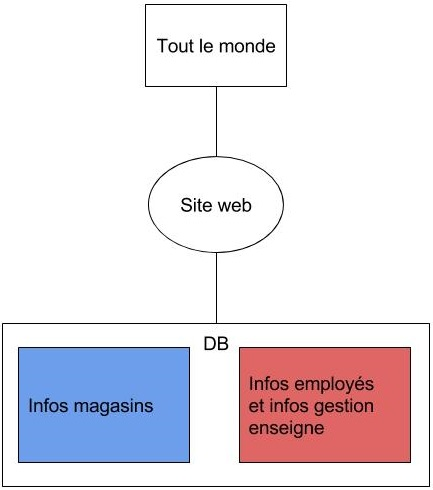
\includegraphics[width=200px]{img/DFD_actuelle.jpg}
\end{center}

Sur ce diagramme de flux, nous pouvons voir que tout le monde accède à toute la base de données du site. En bleu, nous voyons les données qu'un utilisateur et censé pouvoir voir et en rouge, celles auxquelles seul l'administrateur doit pouvoir avoir accès.

\subsection{Menaces}
Comme présenté plus tôt, notre système manque d'un compte admin. Le risque et que n'importe qui (hackers compris) peut accèder aux données des employés et des enseignes. Il pourrait même supprimer les enseignes vu que pour l'instant cette fonctionnalité est offerte à tout le monde via un simple onglet \textbf{Administration}.\\
Voici une liste des menaces potentielles auxquelles notre site peut être confronté.
\begin{itemize}

\item Suppression/Ajout d'enseigne
\begin{itemize}
\item Source: Concurrent, hacker, employé
\item Motivations: Sabotage dans le cas d'un concurrent ou d'un employé en colère. Amusement pour un hacker.
\item Actifs visés: Les enseignes stockées dans la base de données.
\item Potentialité: Forte
\end{itemize}

\item Vue des informations des employés
\begin{itemize}
\item Source:  Employé
\item Motivations: Chantage à propos de salaire. Vol d'informations confidentielles. Spam de masse.
\item Actifs visés: Les salaires stockés dans la base de données.
\item Potentialité: Forte
\end{itemize}

\item Changement du coût des locations
\begin{itemize}
\item Source: Concurrent, hacker
\item Motivations: Sabotage, perte de gains pour l'entreprise ciblée
\item Actifs visés: Les coûts des enseignes dans la base de données
\item Potentialité: Forte
\end{itemize}

\end{itemize}

On voit très vite que le système mis en place actuellement est faible sécuritairement parlant et donc fortement exposé aux menaces. L'analyse de ces dernières nous révèle que c'est la base de données en particulier qu'il faut protéger en parallèle de la connexion admin à implémenter.

\subsection{Scénarios}
Dans cette section nous présenterons certains scénarios probables au vu des menaces décrites plus tôt.

\subsubsection{Sabotage du site web}
Ce scénario va montrer deux des menaces précédemment citées.\\
Bob, qui aime le troll sur internet, tombe sur la page du site. Après la page de choix du centre, il voit alors le bouton \textbf{Administration}. Il a alors accès à toute la gestion des enseignes sur le site. Il peut donc détruire tout ce qui a été mis en place au niveau des enseignes (suppression), mais aussi en ajouter à sa guise. Une attaque du genre, modification des produits plutôt que des enseignes, est survenue l'année passée sur le site d'un grand vendeur français. Nous avons dans ce cas une perte de crédibilité énorme pour le site selon le degré de changements apportés au site.\\
Il peut aussi changer le prix de la location des magasins. Cela serait moins visible mais pourrait faire perdre une masse d'argent considérable si utilisé avec parcimonie (pas de chiffres abérant).

\subsubsection{Vol d'informations des employés}
Jean, employé en colère à cause de son salaire, se rend compte qu'il a accès à la partie \textbf{Administration} du site web de son employeur. Il y trouve toutes les informations à propos de ses collègues (salaire, adresse, ...). Il est donc en détention d'informations privées auxquelles il ne doit absolument pas avoir accès. Il pourrait utiliser cela pour faire du chantage auprès de son patron ou les divulguer pour ternir l'image de l'entreprise.

\subsection{Synthèse}
Nous avons maintenant une bonne vue des problèmes sécuritaires et des menaces de notre système. Il va donc maintenant s'agir de l'améliorer pour le rendre comme ceci:\\
\begin{center}
 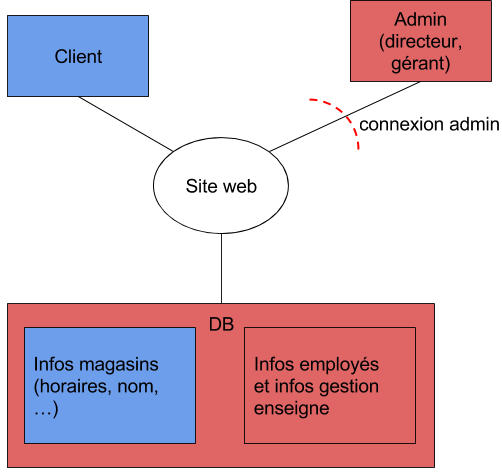
\includegraphics[width=200px]{img/systeme.png}
\end{center}

L'administrateur doit pouvoir accèder à toute la base de données et pouvoir la modifier, l'utilisateur ne doit pouvoir avoir accès qu'aux informations publiques (en bleu). Nous n'allons pas faire de compte entre deux avec un accès sur une partie des informations personnelles (compte employé par exemple).


\section{Mesures sécuritaire}
Dans cette partie, nous allons détailler les mesures sécuritaires entreprises.
\subsection{MySQL}
\begin{itemize}
\item Modification du nom et du mot de passe de l'utilisateur root.
\item Création d'un autre administarteur de la base de donnée avec la philosophie du "moindre privilège", en ne lui accordant que les commande \lstinline{INSERT}, \lstinline{DELETE}, \lstinline{SELECT}, \lstinline{UPDATE}.
\item Supprimer les bases de données inutiles (i.e. \texttt{test}) qui pourrait être des points d'entrées d'attaque.
\item Création d'une table "utilisateurs" avec:
	\begin{itemize}
	\item \texttt{user: String, unique, not null}
	\item \texttt{hash: not null}
	\item \texttt{salt: not null}
	\end{itemize}
    \item \texttt{admin: boolean}, \lstinline{true} si admin.
\item Désactiver \texttt{LOCAL\_INFILE} qui donne un accès au fichiers locaux pour éviter par exemple un affichage de donnée à l'aide d'un \lstinline{SELECT load_file(path)}.
\end{itemize}

\subsection{Frontend/Backend}
\begin{itemize}
\item Lors de requêtes à l'API, demander une authentification pour les routes administrations ("/admin").
\item L'authentification se fait via des Json Web Token avec vérification par signature, grâce à une secret phrase.
\item Stocker la secret phrase dans une variable d'environnement avec un nom non-explicite.
\end{itemize}

Le frontend a été développé en \textbf{Node.js} ce qui nous a grandement facilité la tâche pour améliorer la sécurité de l'application. En effet, des librairies existent déjà, telles que \texttt{json-web-token} et \texttt{express-jwt}.

\texttt{json-web-token} nous a permis de facilement généré un token à partir d'un payload contenant les informations de l'utilisateur. Nous avons aussi ajouté un champ de date de création du token, et fixé une validité d'une heure. Enfin, le module nous a aussi permis de signer le token grâce à une \textit{secret phrase} stockée dans une variable d'environnement.

\begin{lstlisting}{language=HTML,caption=Génération d'un token}
return res.status(200).json(jwt.sign({
	username: data.username,
	exp: exp,
	admin: data.admin
}, config.jwt.secret_key));
\end{lstlisting}

\texttt{express-jwt} est un module permettant de demander une authentification pour accéder à une route de l'API. Une vérification de la signature sera faite et si cette dernière est valide, l'information de l'utilisateur contenue dans le token sera extraite. À partir de ces informations, nous pouvons savoir si l'utilisateur est un administrateur ou pas, et donc lui donner accès à la ressource ou pas.

\subsection{Autres améliorations possibles}
\begin{itemize}
\item Mettre en place un SSL pour une connexion sécurisée. (avec let's encrypt par exemple qui fournit des certificats gratuit et open source).
\end{itemize}

\section{Conclusion}

Ce laboratoire nous a permis de bien comprendre l'impact que pouvait avoir une mauvaise sécurité et comment l'améliorer. Cela nous a aussi permis d'utiliser de nouvelles technologies comme JsonWebToken et de découvrir des modules permettant de gérer la sécurité d'une application web.

\end{document}
